\chapter{Results and Discussion}\label{chapter:res}

\section{Mobile performance}\label{res:performance}

\begin{table}[ht]
	\begin{tabularx}{\textwidth}{X|c|cc|cc}
		\hline
		\multirow{2}{*}{\textbf{\thead{Neural Renderer Configuration}}} 
		& \multirow{2}{*}{\textbf{\thead{Input\\ Layout}}} 
		& \multicolumn{2}{c|}{\thead{\textbf{on GPU (ms)}}}
		& \multicolumn{2}{c}{\thead{\textbf{on DSP (ms)}}} \\ 
		\cline{3-6}
		& 
		& \multicolumn{1}{r|}{\thead{application}}
		& \multicolumn{1}{r|}{\thead{DNN\\alone}}
		& \multicolumn{1}{r|}{\thead{application}}
		& \multicolumn{1}{r}{\thead{DNN\\alone}} \\ 
		\hline
		\thead{ResNet18 encoder, 14.3M params}
		& 2-256-256-4 
		& 55-57
		& 49-50
		& 19--21
		& 19--21 \\
		\hline
		\thead{ResNet18 encoder, 14.3M params}
		& 1-256-256-8 
		& 41--43
		& 38--43
		& 16.6 \underline{cap}
		& 3--4 \\
		\hline
		\thead{MobileNetV3 encoder, 6.7M params}
		& 1-256-256-8 
		& 37--38
		& 30--37
		& 16.6 \underline{cap}
		& 3--4 \\
		\hline
		\thead{MobileNetV3 encoder, 6.7M params}
		& 1-512-512-8
		& 115--136
		& 105--130
		& 21--22
		& 13--14 \\
		\hline
		\thead{ResNet18 encoder, 14.5M params}
		& 1-512-512-8
		& 112--136
		& 105--130
		& 21--22
		& 13--14 \\
		\hline
		\thead{MobileNetV2 encoder, 6.6M params}
		& 1-512-512-8
		& 166--181
		& 150--175
		& 19--21
		& 12--13 \\
		\hline
		\thead{EfficientNet-Lite0 encoder, 6.1M params}
		& 1-512-512-16
		& 71--78
		& 65--75
		& 16.6--17
		& 6--7 \\
		\hline
		\thead{ResNet18 encoder, 14.5M params}
		& 1-640-640-16
		& 200--215
		& 190--200
		& 29--31
		& 28--30 \\
		\hline
	\end{tabularx}	
	\centering
	\caption{Neural Renderer's inference performance, reported for different encoder types, memory layout of input data, when executed on either mobile GPU or DSP devices. The input layout is specified by 4 numbers from left to right: number of OpenGL textures where input frame is rasterized, frame height, frame width, effective number of neural channels stored in a single texture. Since OpenGL textures always have 4 channels, the last number bigger than 4 indicates that quantized 8-bit values are packed into a single texture channel to achieve a contiguous memory layout. The performance of "DNN alone" columns is measured by continuously inferring the DNN with constant random input data, thus excluding: mesh inference, rasterization, output rendering in AR, overall mobile interaction. Application performance has software cap of 60 FPS (16.6 ms).}	\label{res:tab:other-solutions}		
\end{table} 

\section{Quantitative analysis}\label{res:metrics}
\section{Qualitative analysis}\label{res:quality}

\begin{figure}[h!]
	\fboxrule=1pt
	\centering
	\begin{subfigure}[b]{0.495\textwidth}
		\centering
		\cfbox{gray}{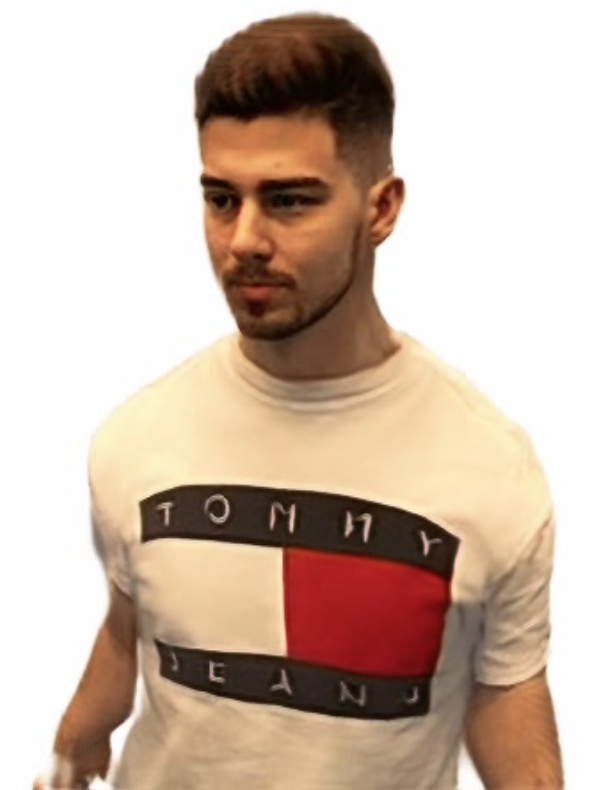
\includegraphics[height=10cm]{\imgfp/example_1}}
		\caption{BNs collect statistics on FB frames}
		\label{res:fig:example}
	\end{subfigure}
	\begin{subfigure}[b]{0.495\textwidth}
		\centering
		\cfbox{gray}{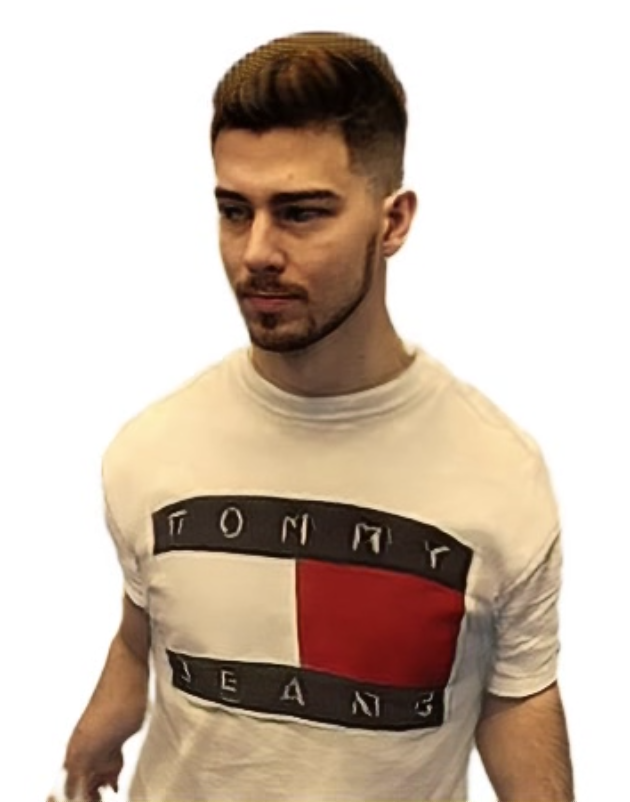
\includegraphics[height=10cm]{\imgfp/example_2}}
		\caption{BNs collect statistics on zoomed frames}
		\label{res:fig:example}
	\end{subfigure}
%	\centering
%	\subcaptionbox{3a\label{fig3:a}}{\includegraphics[width=1.6in]{example-image-c}}\hspace{1em}%
%	\subcaptionbox{3b\label{fig3:b}}{\includegraphics[width=1.6in]{example-image-c}}
	\caption{Example}
	\label{res:fig:example}
\end{figure}
